\newpage
\subsection{Μελέτη του RAS}
\vspace{3mm}

Στο σημείο αυτό μελετάμε την απόδοση του RAS για διαφορες τιμές entries.

\vspace{1em}    
Ακολουθούν τα διαγράμματα που προέκυψαν και ο σχετικός σχολιασμός
τους:

   \begin{minipage}{\textwidth}
      \begin{center}
         \fbox{\textlatin{\textbf{\textit{403-gcc}}}}\\
         \vspace{3mm}
         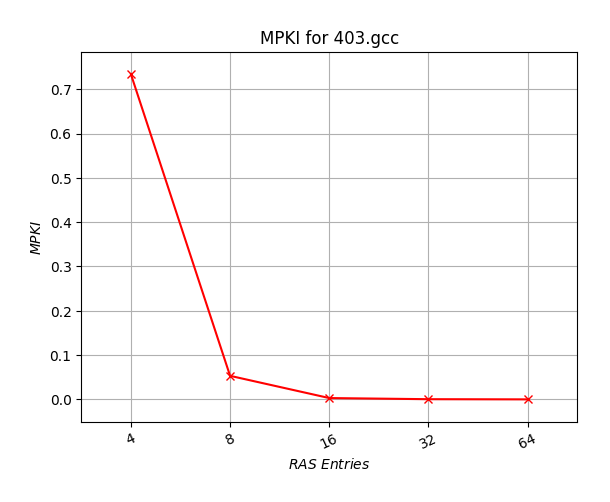
\includegraphics[width=0.65\textwidth, frame]{./graphs/4-4/403-gcc.png}
         \vspace{6mm}
      \end{center}
   \end{minipage}

   \begin{minipage}{\textwidth}
      \begin{center}
         \fbox{\textlatin{\textbf{\textit{429-mcf}}}}\\
         \vspace{3mm}
         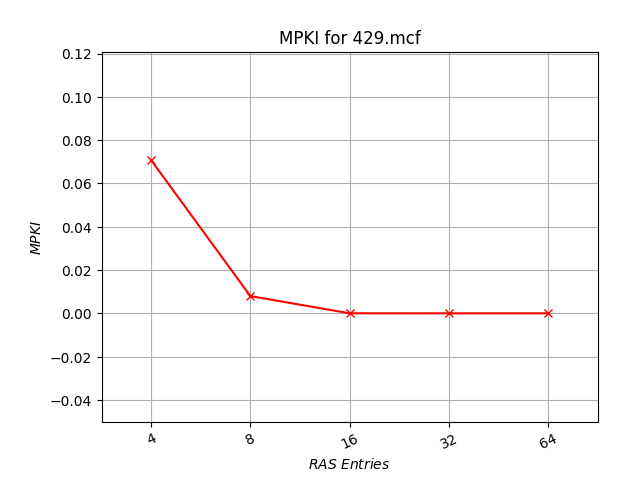
\includegraphics[width=0.65\textwidth, frame]{./graphs/4-4/429-mcf.png}
         \vspace{6mm}
      \end{center}
   \end{minipage}

   \begin{minipage}{\textwidth}
      \begin{center}
         \fbox{\textlatin{\textbf{\textit{434-zeusmp}}}}\\
         \vspace{3mm}
         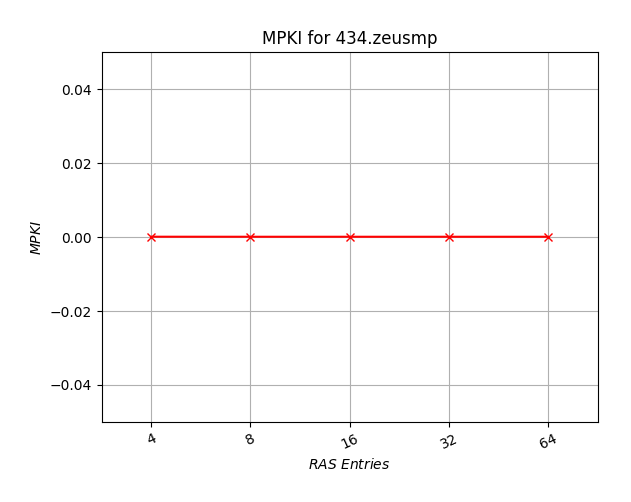
\includegraphics[width=0.65\textwidth, frame]{./graphs/4-4/434-zeusmp.png}
         \vspace{6mm}4
      \end{center}
   \end{minipage}

   \begin{minipage}{\textwidth}
      \begin{center}
         \fbox{\textlatin{\textbf{\textit{436-cactusADM}}}}\\
         \vspace{3mm}
         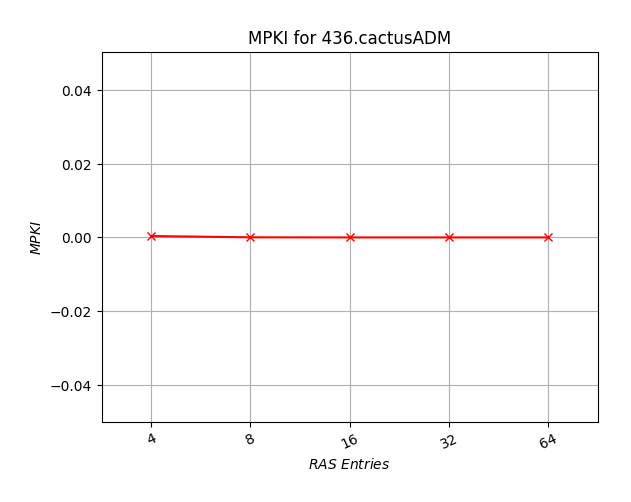
\includegraphics[width=0.65\textwidth, frame]{./graphs/4-4/436-cactusADM.png}
         \vspace{6mm}
      \end{center}
   \end{minipage}

   \begin{minipage}{\textwidth}
      \begin{center}
         \fbox{\textlatin{\textbf{\textit{445-gobmk}}}}\\
         \vspace{3mm}
         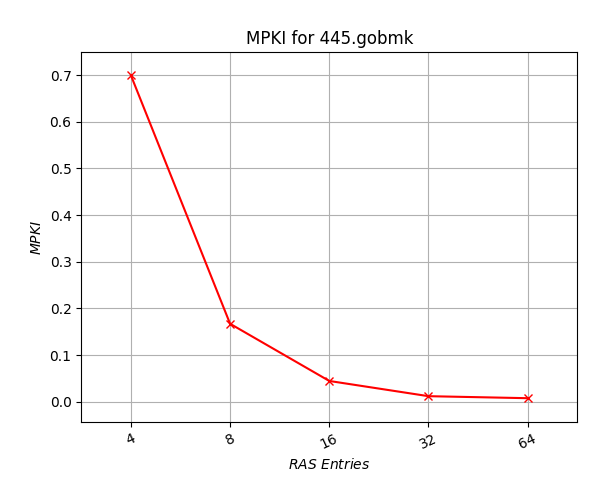
\includegraphics[width=0.65\textwidth, frame]{./graphs/4-4/445-gobmk.png}
         \vspace{6mm}
      \end{center}
   \end{minipage}

   \begin{minipage}{\textwidth}
      \begin{center}
         \fbox{\textlatin{\textbf{\textit{450-soplex}}}}\\
         \vspace{3mm}
         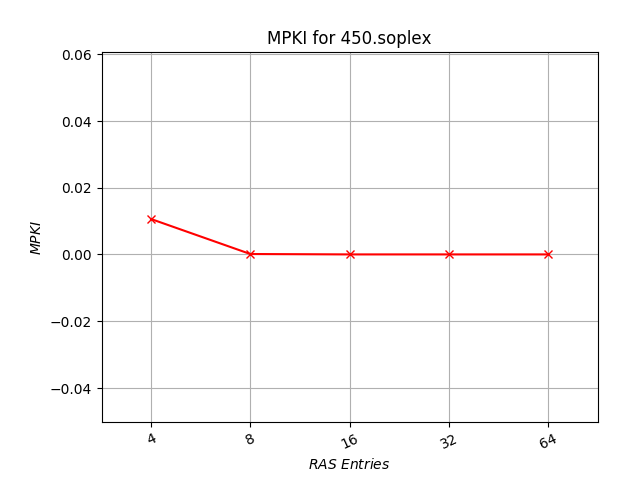
\includegraphics[width=0.65\textwidth, frame]{./graphs/4-4/450-soplex.png}
         \vspace{6mm}
      \end{center}
   \end{minipage}

   \begin{minipage}{\textwidth}
      \begin{center}
         \fbox{\textlatin{\textbf{\textit{456-hmmer}}}}\\
         \vspace{3mm}
         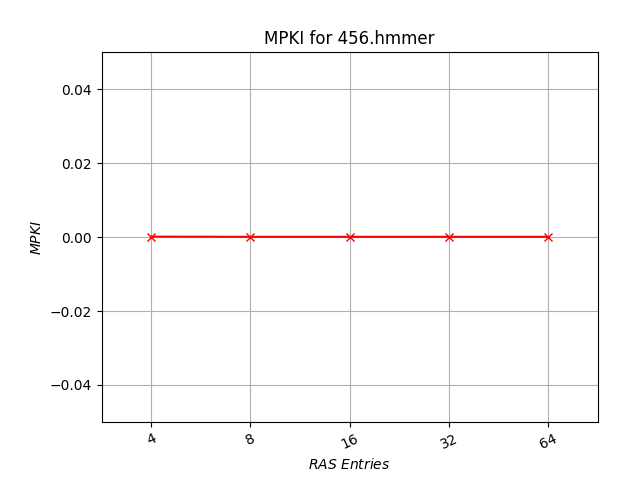
\includegraphics[width=0.65\textwidth, frame]{./graphs/4-4/456-hmmer.png}
         \vspace{6mm}
      \end{center}
   \end{minipage}

   \begin{minipage}{\textwidth}
      \begin{center}
         \fbox{\textlatin{\textbf{\textit{458-sjeng}}}}\\
         \vspace{3mm}
         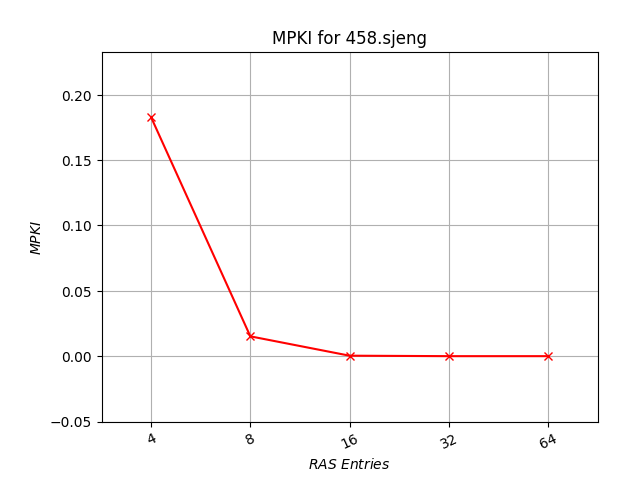
\includegraphics[width=0.65\textwidth, frame]{./graphs/4-4/458-sjeng.png}
         \vspace{6mm}
      \end{center}
   \end{minipage}

   \begin{minipage}{\textwidth}
      \begin{center}
         \fbox{\textlatin{\textbf{\textit{459-GemsFDTD}}}}\\
         \vspace{3mm}
         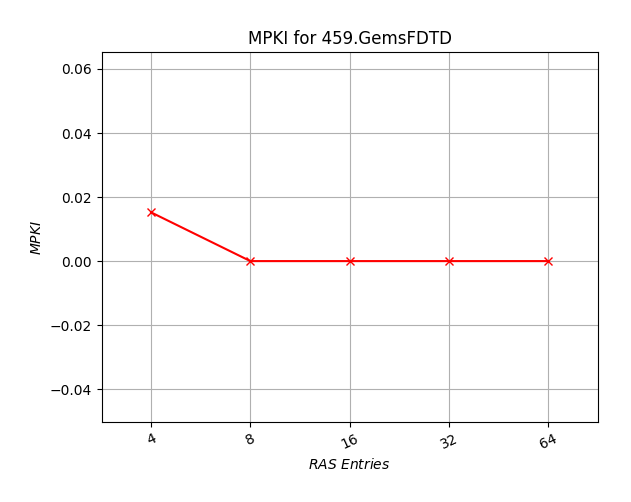
\includegraphics[width=0.65\textwidth, frame]{./graphs/4-4/459-GemsFDTD.png}
         \vspace{6mm}
      \end{center}
   \end{minipage}

   \begin{minipage}{\textwidth}
      \begin{center}
         \fbox{\textlatin{\textbf{\textit{471-omnetpp}}}}\\
         \vspace{3mm}
         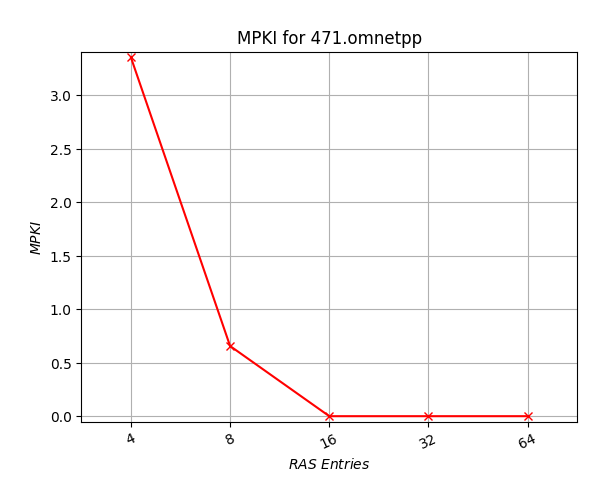
\includegraphics[width=0.65\textwidth, frame]{./graphs/4-4/471-omnetpp.png}
         \vspace{6mm}
      \end{center}
   \end{minipage}

   \begin{minipage}{\textwidth}
      \begin{center}
         \fbox{\textlatin{\textbf{\textit{473-astar}}}}\\
         \vspace{3mm}
         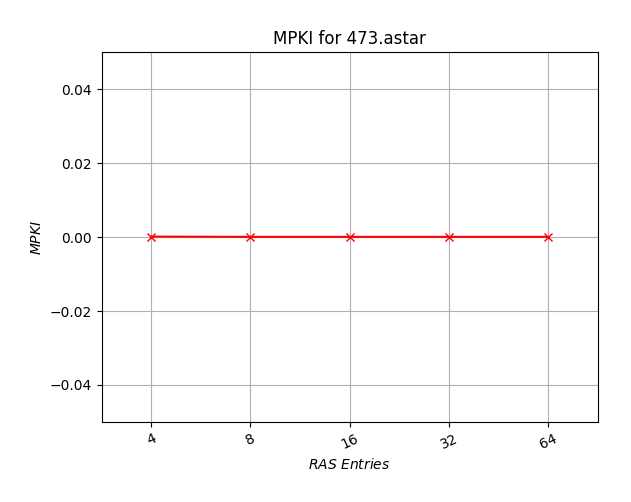
\includegraphics[width=0.65\textwidth, frame]{./graphs/4-4/473-astar.png}
         \vspace{6mm}
      \end{center}
   \end{minipage}

   \begin{minipage}{\textwidth}
      \begin{center}
         \fbox{\textlatin{\textbf{\textit{483-xalancbmk}}}}\\
         \vspace{3mm}
         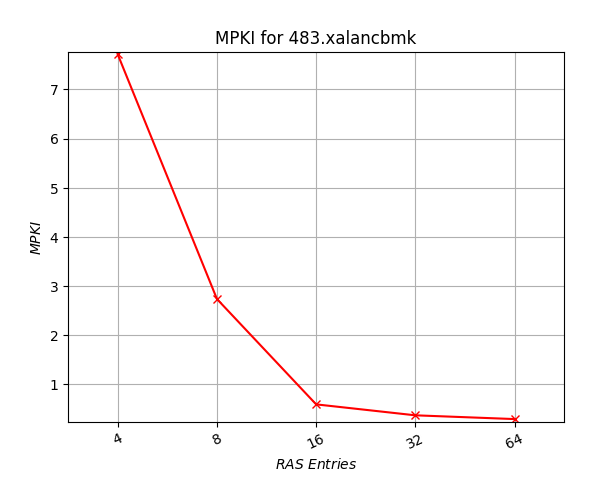
\includegraphics[width=0.65\textwidth, frame]{./graphs/4-4/483-xalancbmk.png}
         \vspace{6mm}
      \end{center}
   \end{minipage}


   \begin{minipage}{\textwidth}
      \begin{center}
         \fbox{\textlatin{\textbf{\textit{Geometric Average of MPKI}}}}\\
         \vspace{3mm}
         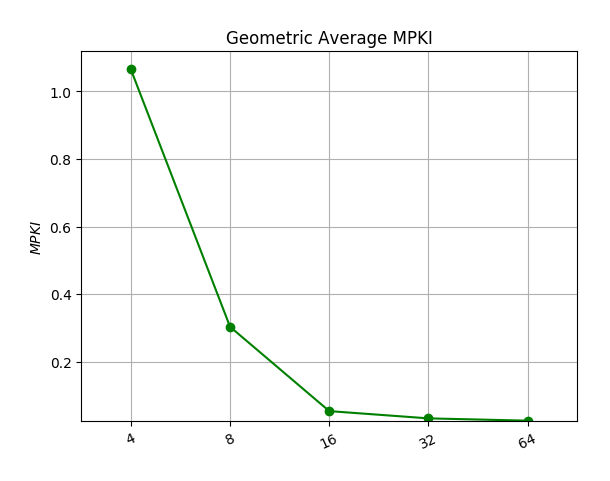
\includegraphics[width=0.65\textwidth, frame]{./graphs/4-4/mean.png}
         \vspace{6mm}
      \end{center}
   \end{minipage}

\paragraph{Συμπεράσματα-Σχόλια}
   

   Για αριθμό εγγραφών στη RAS ίσο με 1, παρατηρούμε σε σχεδόν όλα τα benchmarks
   πολύ υψηλό MPKI. Μόλις το RAS κάνει χρήση 2 εγγραφών, είναι εμφανής η
   σημαντική μείωση του MPKI. Για μεταβολή από 2 σε 4 εγγραφές, παρατηρούμε και
   πάλι σχεδόν σε όλα τα μετροπρογράμματα μείωση του MPKI, όπως είναι επιθυμητό.
   Για παραπάνω entries, τα MPKI είτε μειώνονται με αρκετά μικρότερο ρυθμό, είτε
   παραμένουν σχεδόν σταθερά. Σε κάθε περίπτωση με την αύξηση των εγγραφών οδηγούμαστε
   σε βελτίωση της επίδοσης, ωστόσο από ένα σημείο και πέρα η περεταίρω αύξηση
   δεν έχει νόημα καθώς η επίδοση δεν βελτιώνονται σημαντικά αναλογικά με την
   αύξηση του υλικού που πραγματοποιούμε. 

   Με βάση τα παραπάνω, οι επιλογή 16 ή 32 ή 64 εγγραφών έχει τη βέλτιστη
   επίδοση με κριτήριο αποκλειστικά το MPKI. Ωστόσο, δεν είναι σοφό να
   σπαταλήσουμε extra υλικό (που μεταφράζεται σε κόστος), όταν αυτή η δαπάνη
   υλικού δεν μεταφράζεται σε ανάλογη βελτίωση της απόδοσης. Συνεπώς θα
   επιλέξουμε το ελάχιστο υλικό που επιφέρει την καλύτερη απόδοση. Με βάση το
   κριτήριο αυτό, θα επιλέγαμε τις 16 εγγραφές RAS, καθώς η επίδοση είναι η
   βέλτιστη χωρίς να σπαταλάται hardware. Σε διαφορετική περίπτωση θα μπορούσαμε 
   να επιλέξουμε και τις 8 εγγραφές RAS, με σχετικά μικρή επίπτωση στην απόδοση.
   
   \textbf{Συνοπτικά, καλύτερη επιλογή είναι 16 εγγραφές στην RAS}.